\documentclass{beamer}
%
% Choose how your presentation looks.
%
% For more themes, color themes and font themes, see:
% http://deic.uab.es/~iblanes/beamer_gallery/index_by_theme.html
%
\mode<presentation>
{
	\usetheme{PaloAlto}      % or try Darmstadt, Madrid, Warsaw, ...
	\usecolortheme{whale}
	\setbeamertemplate{footline}[page number] % To replace the footer line in all slides with a simple slide count uncomment this line
} 

\usepackage{graphicx} % Allows including images
\usepackage{booktabs} % Allows the use of \toprule, \midrule and \bottomrule in tables
\usepackage{amsmath}
\usepackage{subfig}
\usepackage{caption}
\usepackage{mathabx}
\usepackage{wrapfig}
\usepackage{tikz}
\usepackage{animate}
\usepackage[english]{babel}
\usepackage[utf8x]{inputenc}
\usepackage{colortbl, booktabs}
\usepackage{multirow}

\usepackage{tikz}
\def\checkmark{\tikz\fill[scale=0.4](0,.35) -- (.25,0) -- (1,.7) -- (.25,.15) -- cycle;} 


\usetikzlibrary{shapes.geometric, arrows}

\title[CB pricing \hspace{0.5cm}\insertframenumber/\inserttotalframenumber]{
Valuing Convertible Bond with Credit Risk Using PDE Model}
\author{Zheng Gao}
\institute{Quantitative Pricing and Risk Analytics\\
QPRA}
\date{14-Dec-2016}


\newcommand\dcdt[2]{\frac{\partial #1}{\partial #2}}



\begin{document}

\begin{frame}
  \titlepage
\end{frame}


\begin{frame}{Outline}
  \tableofcontents
\end{frame}

\section{Introduction}
\begin{frame}{Introduction}{Convertible Bond}
	\begin{itemize}
		\item Hybrid security: a straight bond and a call on the underlying equity
		\item Early conversion, 
			  callability by the issuer, putability by the holder
		\item Components of different risks:
			\begin{itemize}
				\item risk from coupon, principal payments, put provisions
				\item risk free for conversion since the issuer can always deliver its own stock
			\end{itemize}  
		\item Simply using credit spread is not valid: only a part of the Convertible Bond (CB)'s value is exposed to default risk.
		\item Binomial tree method: advantages and disadvantages
	\end{itemize}
\end{frame}

\begin{frame}[shrink=10] {Introduction}{Mathematics Model}
	\begin{itemize}
		\item Proposed by Tsiveriotis and Fernandes in 1998
		\item Defining cash-only part of CB (COCB). Different discounting terms
\begin{equation*}
\textcolor{red}{CB}: \frac{\partial{\textcolor{red}{U}}}{\partial{t}} + 
\frac{\sigma^2S^2}{2}\frac{\partial^2{\textcolor{red}{U}}}{\partial{S}^2} + r_gS\frac{\partial{\textcolor{red}{U}}}{\partial{S}} - r(\textcolor{red}{U}-\textcolor{blue}{V}) - (r+r_c)\textcolor{blue}{V} + P(t) = 0 
\label{eq:CB}
\end{equation*}

\begin{equation*}
\textcolor{blue}{COCB}: \frac{\partial{\textcolor{blue}{V}}}{\partial{t}} + 
\frac{\sigma^2S^2}{2}\frac{\partial^2{\textcolor{blue}{V}}}{\partial{S}^2} + r_gS\frac{\partial{\textcolor{blue}{V}}}{\partial{S}} - (r+r_c)\textcolor{blue}{V} + P(t) = 0 
\label{eq:COCB}
\end{equation*}
	\item Advantage: only needs the \textcolor{red}{market-observed} credit spreads $r_c$ for straight bond of the same issuer.
	\item Other parameters: volatility $\sigma$, risk-free rate $r$, growth rate of the stock $r_g = r - q$, dividend yield $q$ and Coupon payments $P(t)$  
	\end{itemize}
\end{frame}

\begin{frame} {Introduction}{Free Boundary Problem}
	\begin{itemize}
		\item Coupled equations: should be solved simultaneously
		\item Early call, put, and conversion: American-style derivative
		\item Free boundary problem: equations are not valid beyond boundaries
		\item Boundary conditions:
		\begin{equation*}
		\frac{\partial U}{\partial t} = rU + f, \quad S = 0
		\end{equation*}
		\begin{equation*}
		\frac{\partial^2 U}{\partial^2 S} = 0, \quad \textit{large } S
		\end{equation*}
		\item A better way to define the boundary: convert the domain to $[0, 1]$ interval using function 
		$x = \frac{S}{S+\alpha}$, and apply appropriate boundary conditions (Fichera theory).
	\end{itemize}
\end{frame}
\section{Numerical Method}

\begin{frame}{Numerical Method}{Overview}
	\begin{itemize}
		\item Discretizing scheme:
			\begin{itemize}
				\item Explicit scheme: $\Delta t < \frac{1}{\sigma^2}(\frac{\Delta S}{S})^2$, first order in time, second order in space
				\item Implicit scheme: unconditionally stable, first order in time, second order in space
				\item Semi-implicit scheme: unconditionally stable, second order in time and space
			\end{itemize}
		\item Linear solver: projected iteration, apply constraints for each iteration
		\item Adaptive time stepping: depends on the schedule of coupon pay time, print time and change ratio of the solution
	\end{itemize}
\end{frame}

\begin{frame}{Numerical Method}{Implementation}
	\begin{figure}
		\centering
		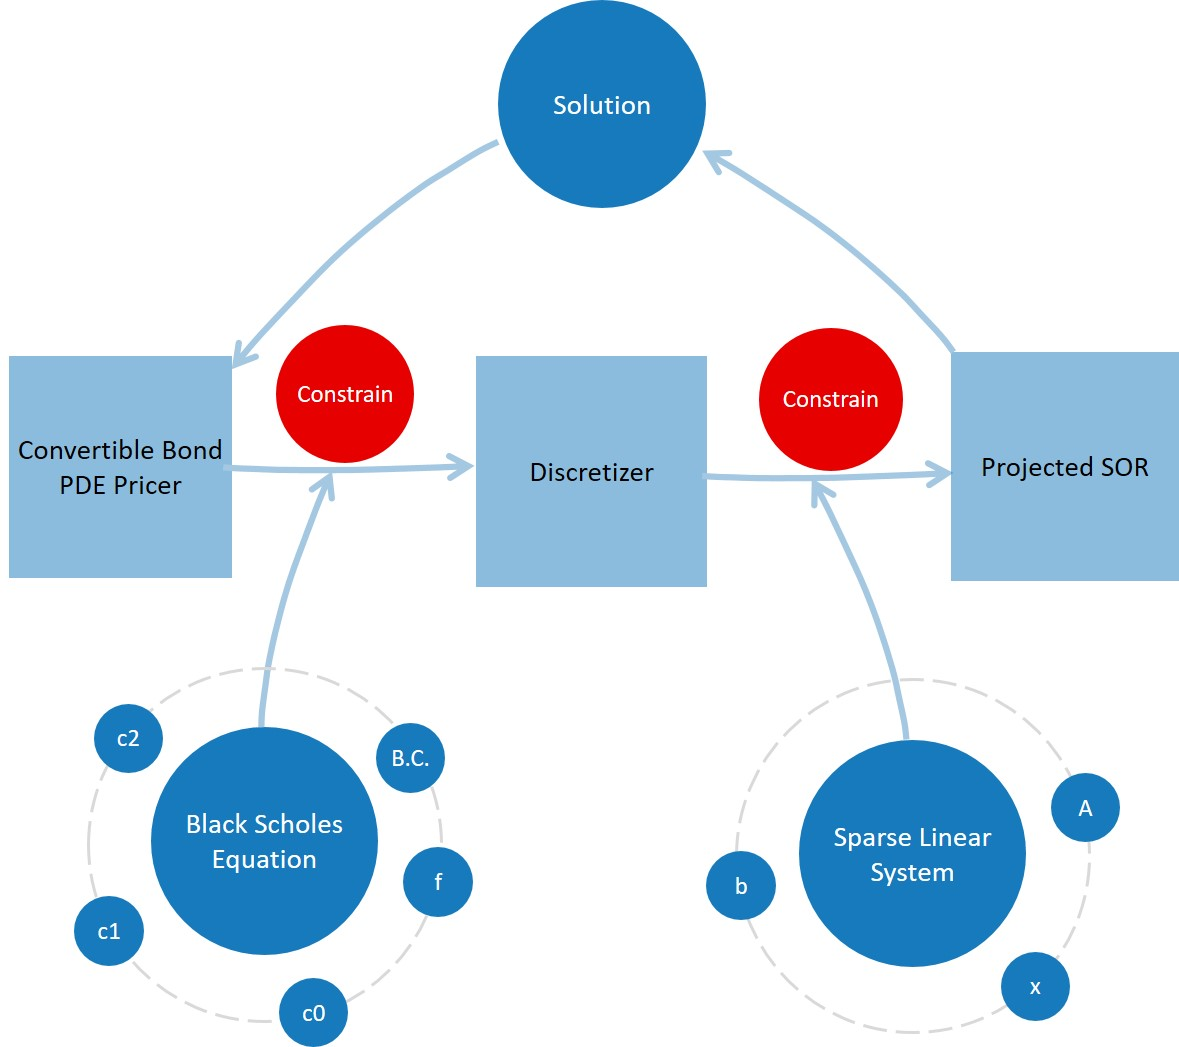
\includegraphics[width=0.75\textwidth]{Figures/Objects}
	\end{figure}
\end{frame}


\section{Numerical Test}

\begin{frame}{Numerical Test}{Parameters}

	\begin{table}
		\centering
		\begin{tabular}{ll}
		\hline\hline\\
		Parameter &  Value \\
		\hline\\
		Volatility & 0.2 \\
		Risk-free interest rate & 0.05\\
		Credit risk & 0.02\\
		Growth rate of stock & 0.02\\
		Time to expiry & 5 \\
		Conversion ratio & 1.0 \\
		Clean call price & 110 from year 2 to year 5\\
		Clean put price & 105 at third year\\
		Coupon payments & \$4, semiannually\\
		\hline
		\end{tabular}
		\caption{Parameters for the test case}
		\label{tb:params}
	\end{table}
	
\end{frame}

\begin{frame}{Numerical Test}{Solution Surface}
	\begin{itemize}
		\item From maturity to initial
		\item Zigzag due to coupon payments
	\end{itemize}
	\begin{figure}
		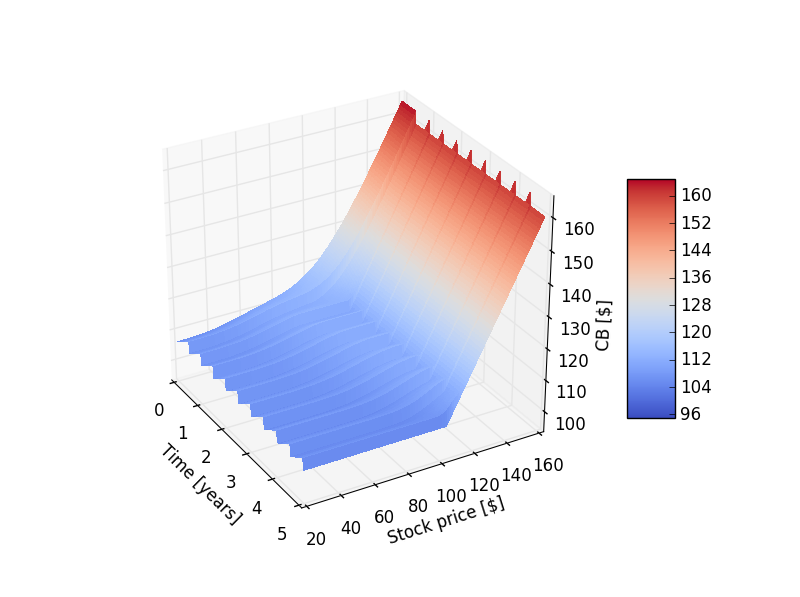
\includegraphics[width=0.5\textwidth]{Figures/CBsurf}
		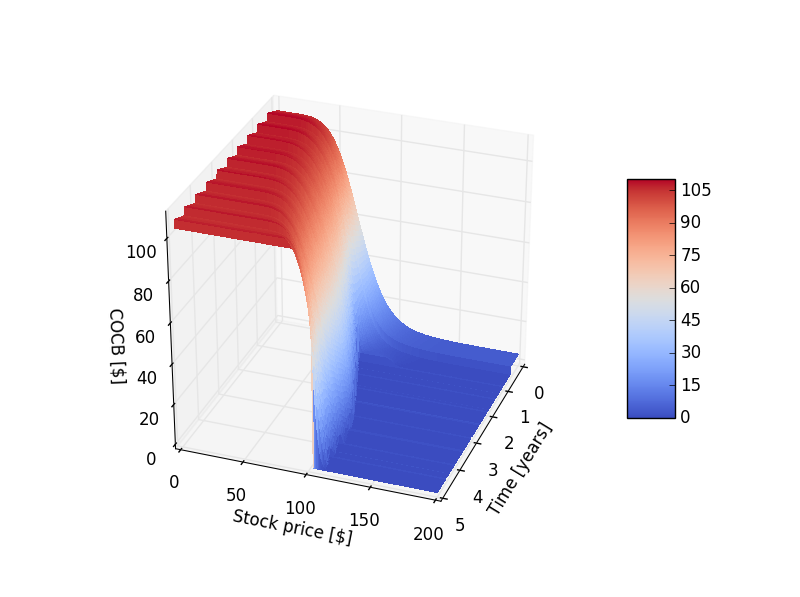
\includegraphics[width=0.5\textwidth]{Figures/COCBsurf}
		\caption{Solution surface for CB (left) and COCB (right)}
		\label{fig:surf}
	\end{figure}
\end{frame}

\begin{frame}{Numerical Test}{Performance}
\begin{itemize}
	\item Time complexity: $\mathcal{O}(N^2)$, linear in time, linear in space
	\item A simulation of $5$ years and grid size of $300$ takes $300 ms$ 
	\begin{figure}
	\centering
	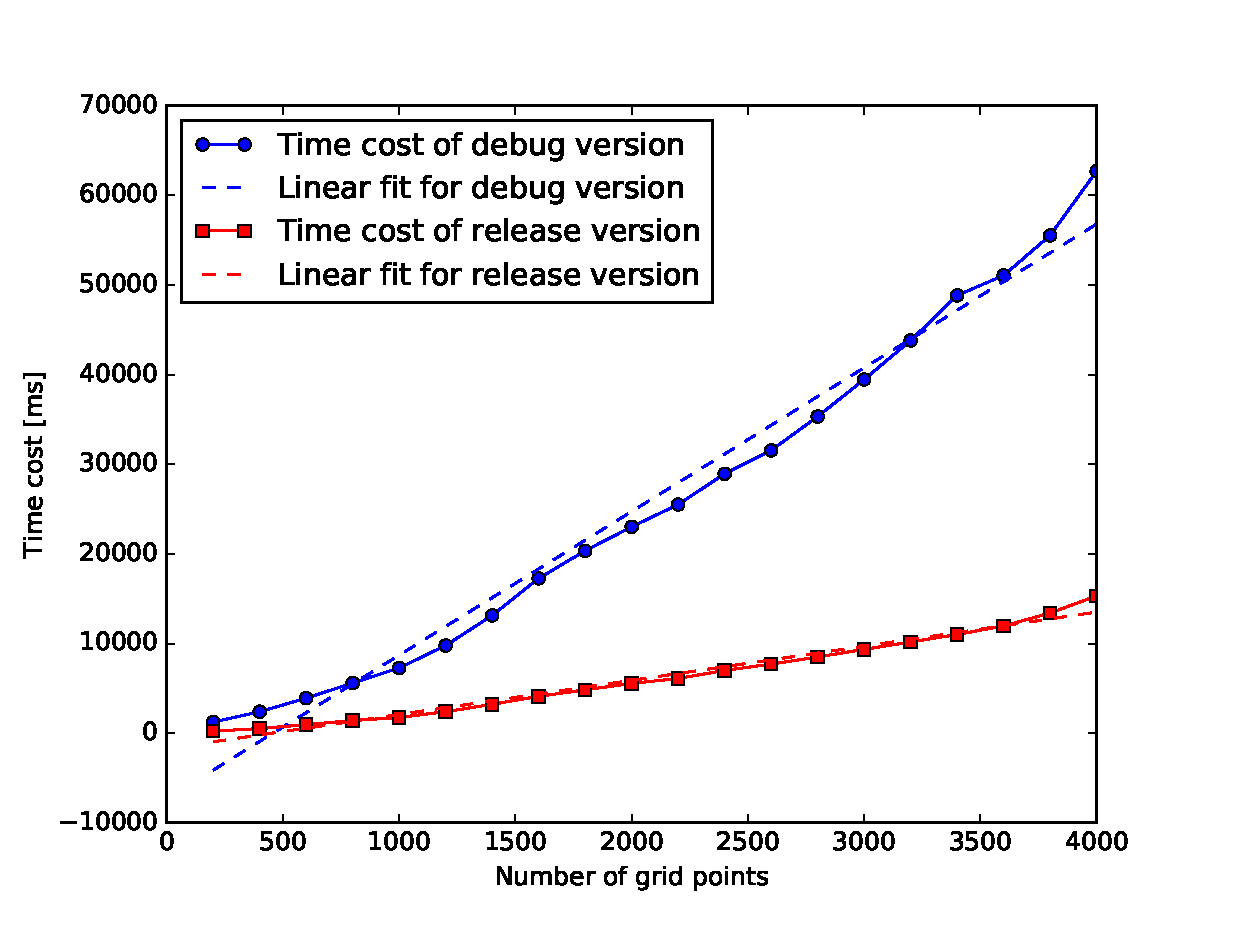
\includegraphics[width=0.8\textwidth]{Figures/timecost}
	\end{figure}
\end{itemize}
\end{frame}

\section{Summary}

\begin{frame}{Summary}{}
\begin{itemize}
	\item Built convertible bond pricer with credit risk using PDE model
	\item Consider conversion, callability, putability and coupon payments
	\item Stable for large time step size, second order in time and space
	\item Future work: Soft call, Foreign exchange volatility(FX)
\end{itemize}
\end{frame}

\begin{frame}{Summary}
	\begin{itemize}
		\item Future work
	\end{itemize}
	\begin{table}
		\centering
		\begin{tabular}{lll}
		\hline\hline\\
		Future/Approach  & Binomial Tree & TF\\
		\hline\\
		Callable		 & \textcolor{blue}{Y} & \textcolor{blue}{Y}\\
		Puttable		 & \textcolor{blue}{Y} & \textcolor{blue}{Y}\\
		Coupon Payments  & \textcolor{blue}{Y} & \textcolor{blue}{Y}\\
		Soft provision   & \textcolor{blue}{Y} & \textcolor{red}{N}\\
		Foreign Exchange & \textcolor{blue}{Y} & \textcolor{red}{N}\\
		Mandatory		 & \textcolor{red}{N} & \textcolor{red}{N}\\
		\hline
		\end{tabular}
		\caption{Comparison between binomial tree and TF model}
		\label{tb:future_work}
	\end{table}
\end{frame}

\section{Appendix}
\begin{frame}{Appendix}{ExcelDNA}
\begin{figure}
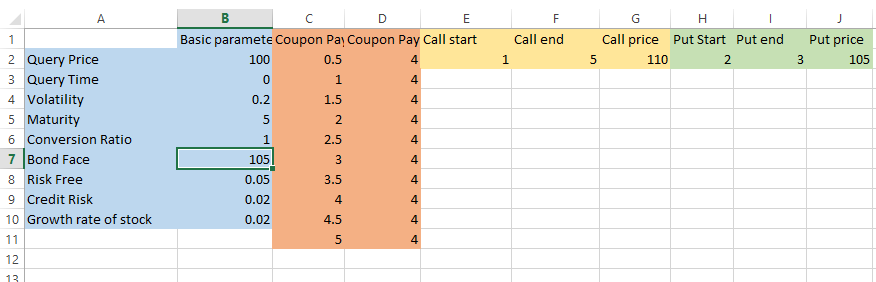
\includegraphics[width=\textwidth]{Figures/excel1.png}\\
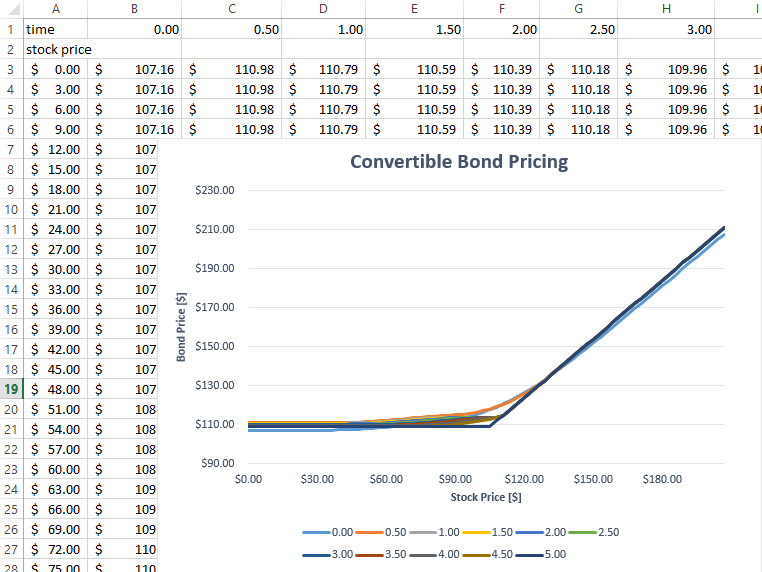
\includegraphics[width=0.25\textwidth]{Figures/excel2.png}
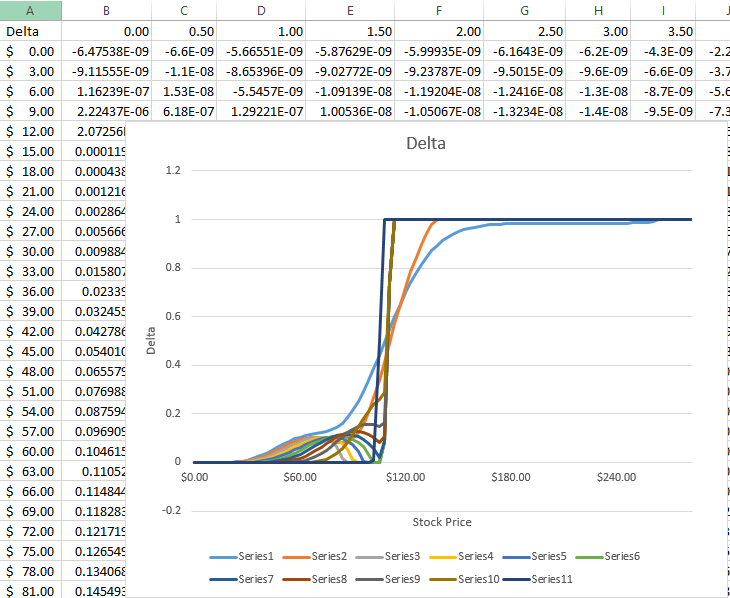
\includegraphics[width=0.25\textwidth]{Figures/excel3.png}
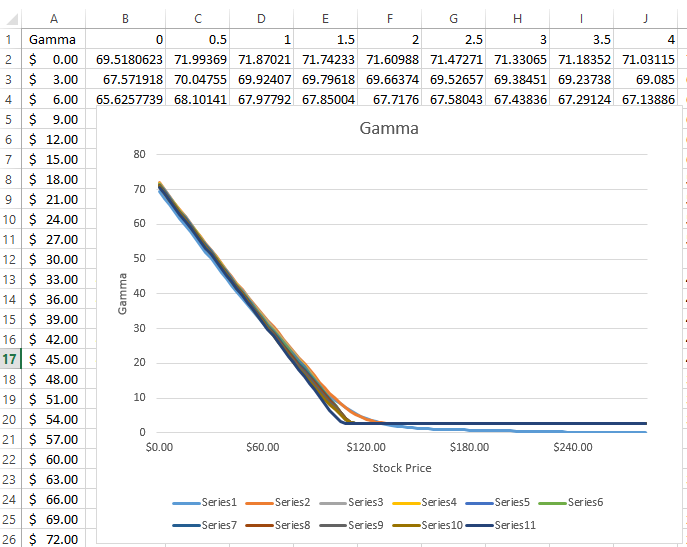
\includegraphics[width=0.25\textwidth]{Figures/excel4.png}
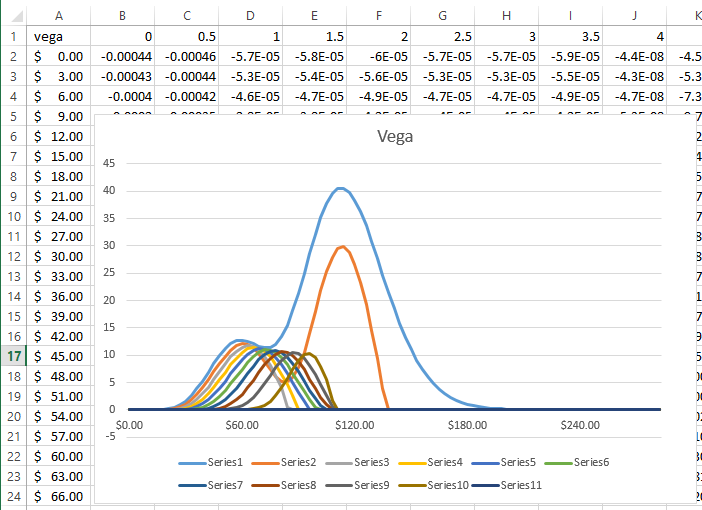
\includegraphics[width=0.25\textwidth]{Figures/excel5.png}
\end{figure}
\end{frame}
\end{document}
